\documentclass[../../relatorio.tex]{subfiles}

\begin{document}


Em decorrência da importância e influência direta no desempenho dos mercados de Seguros, Capitalização e Previdência, os seguintes indicadores serão analisados com mais detalhes
\begin{description}
  \item[Desocupação] Taxa oficial de desemprego no Brasil, divulgado na Pesquisa Mensal do Emprego (PME) pelo IBGE
  \item[Dívida Pública] Dívida pública brasileira medida em relação ao PIB
  \item[IPCA] Inflação oficial medida pelo Instituto Brasileiro de Geografia e Estatística (IBGE)
  \item[Juros] Taxa básica de Juros (SELIC), estipulada mensalmente pelo Comitê de Política Monetária (COPOM) do Banco Central Brasileiro
  \item[PIB] Produto Interno Bruto, divulgado trimestralmente pelo IBGE
  \item[Reservas Internacionais] em USD, divulgados diariamente pelo Banco Central Brasileiro
  \item[IBovespa] Índice da Bolsa de Valores de São Paulo (Bovespa)
  \item[Câmbio] das principais moedas extrangeiras - USD, EUR e GBP
  \item[EMBI+Br] Risco Brasil, divulgado diariamente pela Standard and Poors
  \end{description}

\section{Painel Macroeconômico}

%No mês de Maio de 2015 muda.
% latex table generated in R 3.1.1 by xtable 1.7-4 package
% Tue Jul 28 19:11:12 2015
\begin{table}[ht]
\centering
\begin{tabular}{ll}
   \hline
Taxa de Desemprego & 6.7\% em 2015/05 \\ 
  Dívida Pública & 66.8\% do PIB em 2015/05 \\ 
  Inflação oficial acum. em 12 meses & 8.88\% em 2015/06 \\ 
  Taxa básica de Juros (SELIC/Bacen) & 13.65\% (a.a.) em 2015/07 \\ 
  Produto Interno Bruto & 1.408 BRL Trilhões em 2015/01 \\ 
  Reservas Internacionais (Bacen) & 368 USD Bilhões em 15/07/2015 \\ 
  IBovespa & 53070 pontos 16/07/15 \\ 
  EUR 1.00 & 3.4266 BRL em 17/07/2015 \\ 
  USD 1.00 & 3.1407 BRL em 17/07/2015 \\ 
  GBP 1.00 & 4.9045 BRL em 17/07/2015 \\ 
  Risco País (EMBI+ Brasil) & 306 bp (100 bp = 1\%) em 15/07/2015 \\ 
   \hline
\end{tabular}
\caption{Principais indicadores macroeconômicos} 
\end{table}
\pagebreak

\begin{figure}[ht]
  \begin{minipage}{0.70\textheight}
    \centering
      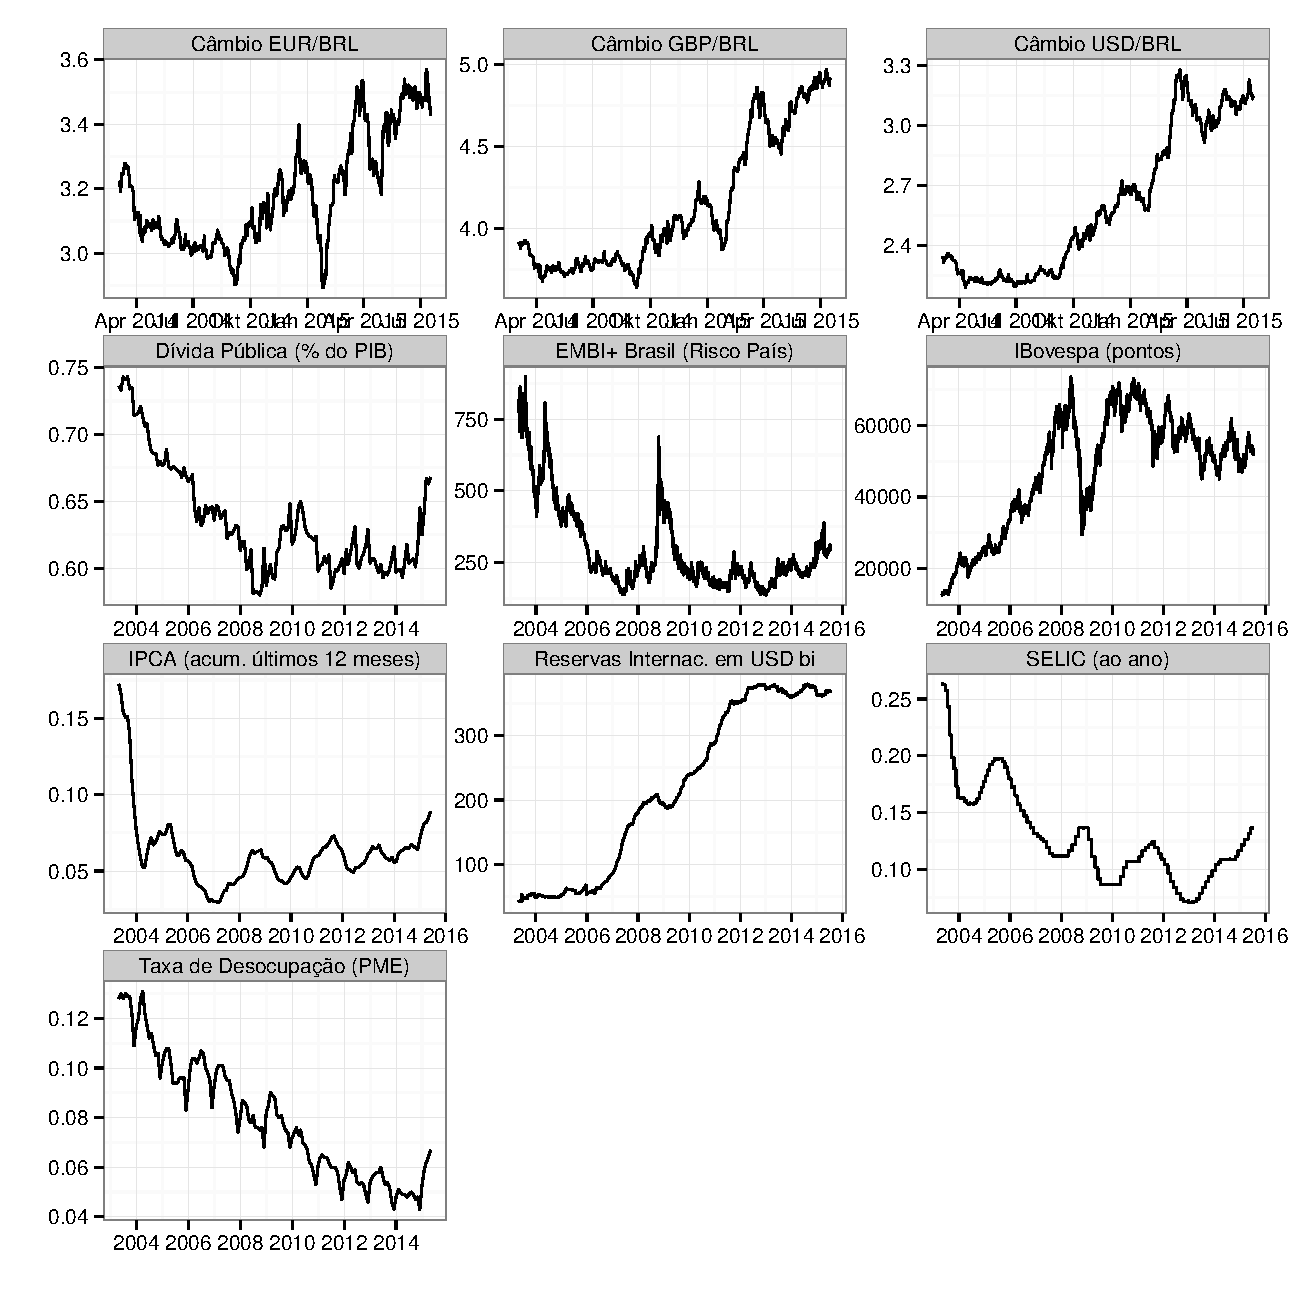
\includegraphics[width=0.7\textheight]{PainelMacro.pdf}
  \end{minipage}
\end{figure}

\end{document}
